% Generated by julia/scripts/solve_unified_canonical_benchmark.jl.
% Source: experiments/results/summaries/unified_canonical_transition_edges.csv.
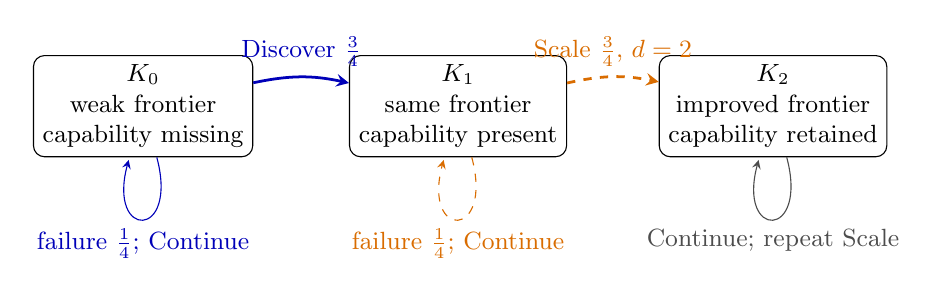
\begin{tikzpicture}[>=stealth,font=\small]
  \node[draw,rounded corners,align=center,minimum width=2.3cm] (k0) at (0,0)
    {\(K_0\)\\weak frontier\\capability missing};
  \node[draw,rounded corners,align=center,minimum width=2.3cm] (k1) at (4,0)
    {\(K_1\)\\same frontier\\capability present};
  \node[draw,rounded corners,align=center,minimum width=2.3cm] (k2) at (8,0)
    {\(K_2\)\\improved frontier\\capability retained};
  \draw[->,blue!72!black,line width=1.0pt]
    (k0) to[bend left=12] node[above] {Discover \(\frac{3}{4}\)} (k1);
  \draw[->,orange!85!black,dashed,line width=1.0pt]
    (k1) to[bend left=12] node[above] {Scale \(\frac{3}{4}\), \(d=2\)} (k2);
  \draw[->,blue!72!black]
    (k0) edge[loop below] node {failure \(\frac{1}{4}\); Continue} (k0);
  \draw[->,orange!85!black,dashed]
    (k1) edge[loop below] node {failure \(\frac{1}{4}\); Continue} (k1);
  \draw[->,black!70]
    (k2) edge[loop below] node {Continue; repeat Scale} (k2);
\end{tikzpicture}
